\documentclass{article}

\usepackage[utf8]{inputenc}
\usepackage{graphicx}   % Para imágenes.
\usepackage{multicol}
\usepackage{amsmath}
\usepackage{dashrule}
\usepackage{geometry}
\usepackage[spanish, mexico]{babel}
\usepackage{subcaption}
\usepackage[svgnames]{xcolor}
\usepackage{tcolorbox}
\usepackage[table,xcdraw]{xcolor}
\usepackage{fancyhdr}
\usepackage{enumitem}
\usepackage{siunitx}
\usepackage[export]{adjustbox}
\usepackage{multirow}


\usepackage[normalem]{ulem}
\useunder{\uline}{\ul}{}

\definecolor{gray(x11gray)}{rgb}{0.75, 0.75, 0.75}
\definecolor{outerspace}{rgb}{0.25, 0.29, 0.3}
\definecolor{pastelgreen}{rgb}{0.47, 0.87, 0.47}
\definecolor{lincolngreen}{rgb}{0.11, 0.35, 0.02}

\geometry{
    a4paper,
    tmargin = 1.7 cm,
    bmargin = 1.7cm,
    lmargin = 1.5cm,
    rmargin = 1.5cm
}



\pagestyle{fancy}
\fancyhf{}
\cfoot{ \thepage  \hspace{0.5pt}\hspace{0.5pt}}
\lhead{Tarea Examen}

\begin{document}

\thispagestyle{plain}


\hrule
\begin{center}
    {\Large \textbf{UNIVERSIDAD NACIONAL AUTÓNOMA DE MÉXICO}}
    \vspace{10pt}

    {\Large{{Sistemas hibridos en biomedicina}}}
    
    
    \vspace{10pt}

    \hrule

    \vspace{20pt}


    {\Huge \textbf{Tarea 3: Suministro de energía}}\\
\end{center}

\hdashrule{\linewidth}{1pt}{1mm}

\begin{flushright}
    {\small Medel Garduño Diego} 
\end{flushright}

\section{Sistema de alimentación de CT}


Cuando se habla de un sistema de tomografia axial computarizada, se debe considerar la parte del gantry, elemento que esta en continua rotación, este hecho puede provocar distintas problematicas, ya que para que tenga alimentación debe hace uso de cables que pueden enrrollarse con el movimiento, para solucionar este problema se hace uso de anillos colectores de energía, los cuales son sistemas que mantienen en continua conexión una parte movil y una parte fija. [\textcolor{blue}{1}]


\vspace{10pt}

\begin{figure}[h!]
    \centering
    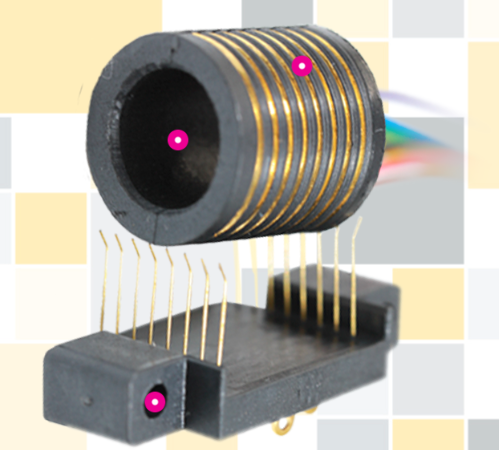
\includegraphics[scale = 0.40]{rotor.png}
    \caption{Interior de un anillo colector electrico}
    \label{t1}
\end{figure}


\vspace{10pt}

En la figura \ref{t1} se muestra un diagrama del interior de un anillo colector electrico, que esta conformado por un cilindro rodeado de anillos hechos de material conductor, este cilindro es la unidad movil. Mientras que debajo del anillo se encuentra la unidad estatica, que esta formada por un cepillo con cerdas de material conductor. Los anillos del cilindro se mantienen en contacto constante con el cepillo, de esta forma se permite que haya rotación evitando los problema asociados a cables. [\textcolor{blue}{1}]
Este sistema es a microescala considerando las dimensiones asociadas a un tomografo, sin embargo es el mismo principio, los cables de alimentación que vienen de la acometida se conecta al elemento estatico del anillo colecto, este alimenta al cilidro movil, el cual a su vez, alimenta al gantry que es la parte que movil de un tomografo. 

\vspace{10pt}


Estos equipos deben cumplir con normas especificas de la Comisión Electrotécnica Internacional (IEC), como las siguientes: [\textcolor{blue}{2}]


\begin{enumerate}
    \item Norma IEC 601-1
    \item Norma IEC 60601-2-44
    \item Norma IEC 601-1.18
\end{enumerate}

\section{Diferencia entre multiespetral e hiperespectral}


Para entender esta diferencia se debe comprender en principio lo que es una imagen espectral, la cual en una definición robusta es aquella que muestra las distintas longitudes de ondas en el espectro electromagnetico emitidas por un objeto. De estas imagenes se desprenden dos visiones, la multiespectral y la hiperespectral. [\textcolor{blue}{3}]


\begin{figure}[h!]
    \centering
    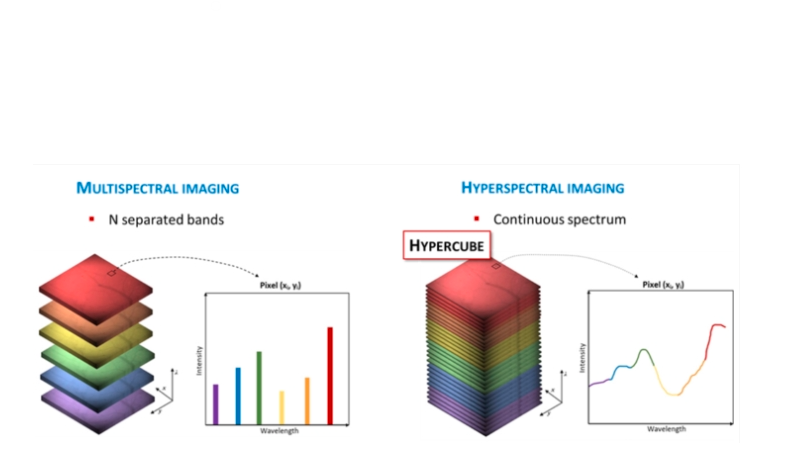
\includegraphics[scale = 0.60]{hiper.png}
    \caption{Diferencia entre multiespectral e hiperespectral}
    \label{t1}
\end{figure}


La vision multiespectral se refiere a aquella en la que se utilizaron un número discreto de bandas para formar el espectro visto en una imagen espectral. De manera comun se consideran las bandas del rojo, azul y verde, en ocasiones especificas se puede considerar el infrarrojo cercano o termico. Por otro lado la visión hiperespectral no esta limitada a un rango de bandas, sino que considera un rango más amplio, esta visión no solo considera bandas especificas, sino que puede llegar a comtemplar bandas en el rango de millones, dando información desde el ultravioleta hasta el infrarrojo lejano. [\textcolor{blue}{4}] 


\section*{Referencias}

\begin{enumerate}
    \item [[\textcolor{blue}{1}]] Rota-RX. (2024). Tecnología médica. Recuperado de https://www.rotarx.com/es/aplicaciones/tecnologia-medica/
    \item [[\textcolor{blue}{2}]] Vaca Bastidas, E. I. (2002). Guía técnica de instalación, ajuste, y puesta en marcha de un equipo de tomografía axial computarizada (Tesis de grado, Escuela Politécnica Nacional). Escuela Politécnica Nacional.
    \item [[\textcolor{blue}{3}]] Grupo Álava. (2024). ¿Qué diferencia una imagen multiespectral de una hiperespectral? Grupo Álava. https://www.grupoalava.com/ingenieros/actualidad/que-diferencia-una-imagen-multiespectral-de-una-hiperespectral/
    \item [[\textcolor{blue}{4}]] Multiespectral.es. (s.f.). Diferencias entre visión multiespectral e hiperespectral. Recuperado de https://multiespectral.es/diferencias-entre-vision-multiespectral-e-hiperespectral
\end{enumerate}

\end{document}